\documentclass[conference]{IEEEtran}
\IEEEoverridecommandlockouts
\usepackage{cite}
\usepackage{amsmath,amssymb,amsfonts}
\usepackage{algorithmic}
\usepackage{graphicx}
\usepackage{textcomp}
\usepackage{xcolor}
\usepackage{threeparttable}
\usepackage{float}
\usepackage{hyperref}

\floatstyle{boxed} 
\restylefloat{figure}

\def\BibTeX{{\rm B\kern-.05em{\sc i\kern-.025em b}\kern-.08em
    T\kern-.1667em\lower.7ex\hbox{E}\kern-.125emX}}
\begin{document}

\title{Sleep State Prediction Using Accelerometry Data: A Systematic and Computational Approach}

\author{
	\IEEEauthorblockN{Juan Carlos Quintero Rubiano}
	\IEEEauthorblockA{Code: 20232020172\\
		\textit{Systems Engineering} \\
		\textit{Francisco Jose de Caldas District University}\\
		Bogota, Colombia \\
		jcquineror@udistrital.edu.co}\\
	%and
	\IEEEauthorblockN{Juan Felipe Wilches Gomez}
	\IEEEauthorblockA{Code: 20231020137\\
		\textit{Systems Engineering} \\
		\textit{Francisco Jose de Caldas District University}\\
		Bogota, Colombia \\
		jfwilchesg@udistrital.edu.co}
	\and
	\IEEEauthorblockN{Juan Nicolas Diaz Salamanca}
	\IEEEauthorblockA{Code: 20232020059\\
		\textit{Systems Engineering} \\
		\textit{Francisco Jose de Caldas District University}\\
		Bogota, Colombia \\
		jndiazs@udistrital.edu.co}
}

\maketitle

\begin{abstract}
	Sleep is a complex physiological process composed of several distinct states, each playing a critical role in health and well-being. Traditional measurement of sleep states relies on polysomnography, an expensive and intrusive method. Recent advances in wearable technology have enabled the use of accelerometers as a non-invasive, low-cost alternative for sleep state prediction. This paper presents a systematic analysis and computational approach for predicting sleep states using accelerometry data, focusing on the extraction of movement patterns and temporal features. We discuss the theoretical background, computational models, and methodological considerations, highlighting the potential and limitations of accelerometer-based sleep monitoring.
\end{abstract}

\begin{IEEEkeywords}
	Sleep states, accelerometry, computational models, wearable devices, sleep monitoring, time series analysis.
\end{IEEEkeywords}

\section{Introduction}

Sleep is a fundamental biological process essential for physical and mental health, comprised of distinct states: light sleep (N1, N2), deep sleep (N3), REM sleep, and wakefulness~\cite{carskadon2005normal, diekelmann2010sleep}. Each state serves specific physiological functions—deep sleep facilitates physical restoration and memory consolidation, while REM sleep supports emotional processing and learning~\cite{diekelmann2010sleep}. These states were systematically defined by Rechtschaffen and Kales~\cite{rechtschaffen1968} and later refined by the American Academy of Sleep Medicine~\cite{aasm2007}.

Sleep disorders affect a significant portion of the population, manifesting as disruptions to normal sleep patterns. Accurate identification of sleep states is crucial for diagnosing these disorders and evaluating treatment efficacy. Traditionally, sleep monitoring relies on polysomnography (PSG), which records multiple physiological signals (EEG, EOG, EMG)\footnote{EEG (Electroencephalogram): Records brain electrical activity. EOG (Electrooculogram): Measures eye movements, essential for REM detection. EMG (Electromyogram): Records muscle activity, crucial for identifying muscle atonia during REM sleep.} in specialized laboratories~\cite{aasm2007}. While PSG remains the gold standard, its cost, complexity, and laboratory setting limit widespread application and can disrupt natural sleep patterns~\cite{pmc5781106}.

Recent advances in wearable technology have enabled the use of accelerometers as a non-invasive, low-cost alternative for sleep state prediction. These sensors, embedded in consumer devices like smartwatches and fitness trackers, measure body movement to infer sleep and wake states~\cite{pmc4883440, sadeh2011}. The validity and reliability of accelerometry have been evaluated against polysomnography, with studies confirming its utility for sleep/wake discrimination~\cite{littner2003, kushida2001}, though limitations remain in distinguishing specific sleep stages.

The widespread availability of these devices has democratized access to sleep monitoring and motivated the development of sophisticated computational models to bridge the gap between consumer wearables and clinical assessment tools. This paper addresses the central question: \textit{How can accelerometer data be used to accurately predict sleep states?}

\section{Theoretical Framework: Computational Models for Sleep State Prediction}

Computational models for sleep state prediction from accelerometry data typically involve time series analysis, feature extraction, and classification algorithms. The underlying assumption is that movement patterns correlate with different sleep states: periods of low movement are associated with sleep, while increased activity indicates wakefulness~\cite{pmc4883440, researchgate2021, sadeh2011}. This approach is grounded in the established understanding of sleep physiology and regulation, such as the Two-Process Model proposed by Borbely~\cite{borbely1982}, which describes the interaction between homeostatic sleep drive (Process S) and circadian rhythm (Process C) in regulating sleep-wake cycles.

Sleep state classification techniques have evolved from the manual scoring rules first proposed by Rechtschaffen and Kales in 1968~\cite{rechtschaffen1968}, which established standardized criteria for identifying sleep stages based on polysomnography recordings. These were later refined by the American Academy of Sleep Medicine (AASM)~\cite{aasm2007}, which introduced the current terminology of N1, N2, N3 (replacing stages 1-4), and REM sleep. While accelerometry lacks the neurophysiological signals needed for precise staging according to these criteria, computational approaches seek to approximate sleep state classification through movement pattern analysis.

Common approaches include:
\begin{itemize}
	\item \textbf{Threshold-based algorithms:} These use simple rules based on movement intensity to distinguish sleep from wake. For example, the Sadeh and Cole-Kripke algorithms are widely used in actigraphy-based sleep scoring~\cite{van2011review, sadeh2011}.
	\item \textbf{Machine learning models:} Supervised classifiers such as random forests, support vector machines, and logistic regression are trained on labeled data to improve classification accuracy~\cite{van2011review, zhang2020machine, vanHees2015}.
	\item \textbf{Deep learning:} Recurrent neural networks (RNNs), convolutional neural networks (CNNs), and hybrid models are increasingly used to capture temporal dependencies and complex patterns in accelerometry data~\cite{zhang2020machine, behar2013}.
\end{itemize}

The accuracy of these models depends on the quality of the input data, feature engineering, and the availability of ground truth labels, often derived from PSG. While accelerometer-based systems are effective for distinguishing sleep from wake, their ability to differentiate between specific sleep stages (e.g., REM vs. non-REM) is limited compared to PSG~\cite{pmc4883440, researchgate2021, kushida2001, griessenberger2013}.

\section{Methods and Materials: Systematic Analysis Using Accelerometry Data}

\subsection{Data Source}
The primary data source is the accelerometer, which measures wrist movement in three axes. No environmental or physiological data (e.g., light, temperature, EEG) are available in this analysis. This limitation is common in wearable-based sleep monitoring systems~\cite{researchgate2021}.

\begin{figure}[h]
	\centering
	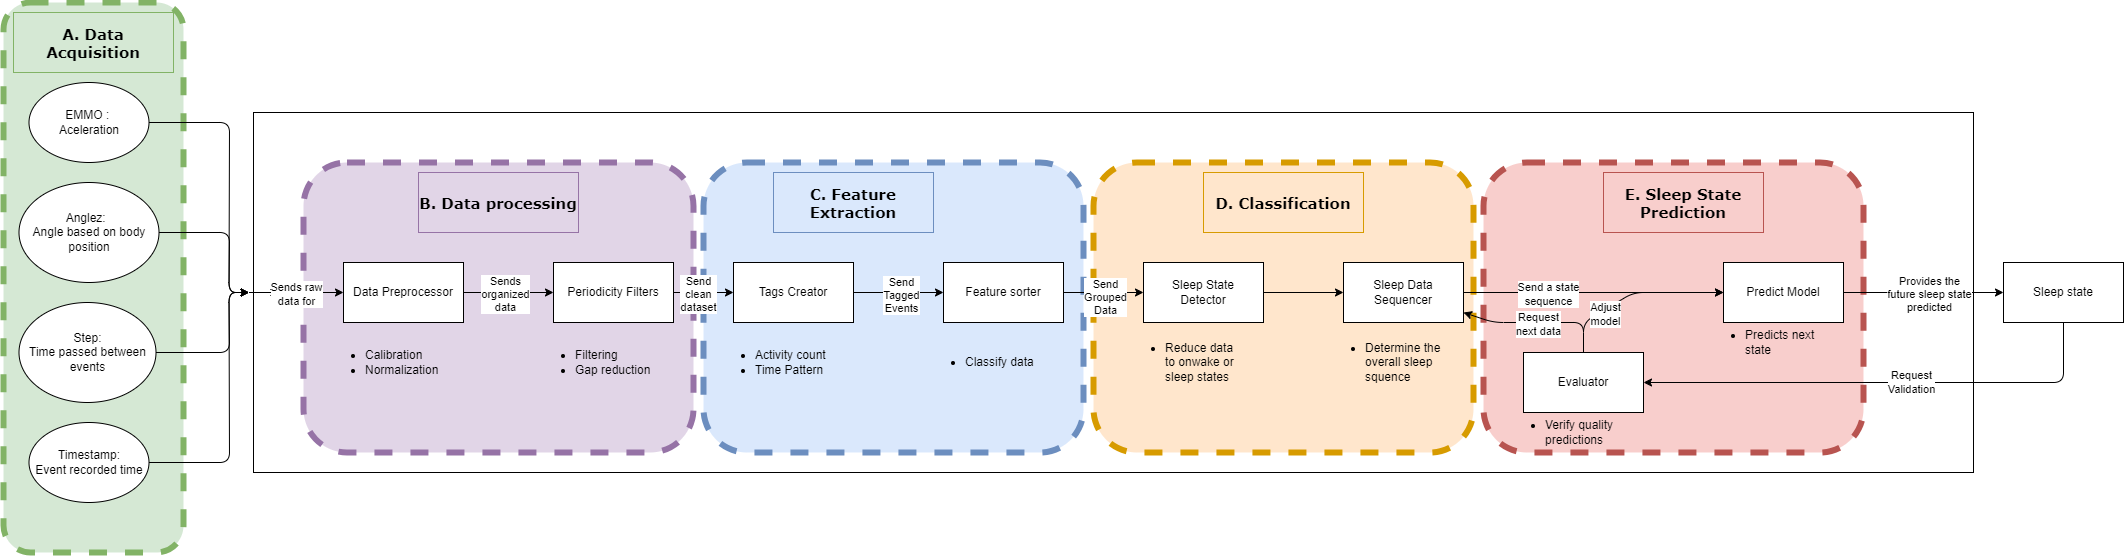
\includegraphics[width=0.3\linewidth]{figures/conceptual_model.png}
	\caption{Conceptual model of sleep state classification using accelerometer data. The pipeline processes raw accelerometer signals through multiple stages: (A) Data acquisition from wrist-worn device, (B) Signal preprocessing and noise removal, (C) Feature extraction across time and frequency domains, (D) Classification using machine learning models, and (E) Prediction of sleep/wake states across time. \textit{Figure created using AI.}}
	\label{fig:conceptual_model}
\end{figure}

\subsection{Variables Analyzed}
\begin{itemize}
	\item \textbf{Wrist movement:} Intensity and temporal patterns of movement, as measured by the accelerometer.
	\item \textbf{Movement speed:} Changes in velocity over time, derived from the raw acceleration data.
	\item \textbf{Timestamp:} Used to sequence movement data and analyze temporal patterns. The timestamp is also useful for inferring environmental conditions, such as likely periods of darkness (nighttime), which are associated with sleep.
\end{itemize}

Although brain activity at rest is a key indicator of sleep, it is not directly measured by accelerometers. Instead, periods of minimal movement are used as a proxy for sleep states~\cite{pmc5781106}. The absence of movement, especially during expected sleep periods, is interpreted as sleep, while increased activity is interpreted as wakefulness.

\subsection{Polysomnography vs. Accelerometry}

Polysomnography (PSG) is the gold standard for sleep assessment, providing comprehensive recordings of biophysiological changes during sleep~\cite{rechtschaffen1968, aasm2007}. PSG simultaneously monitors multiple parameters including EEG (brain activity), EOG (eye movements), EMG (muscle tone), ECG (heart rate), and respiratory parameters.

\begin{figure}[h]
	\centering
	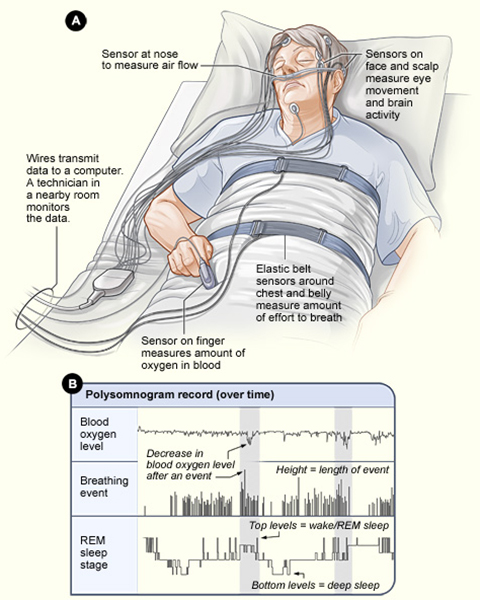
\includegraphics[width=0.5\linewidth]{figures/psg_setup_diagram.png}
	\caption{Polysomnography setup showing the arrangement of multiple sensors for comprehensive sleep monitoring. Key components include: EEG electrodes (positioned according to the international 10-20 system), EOG electrodes for detecting eye movements, EMG electrodes for measuring muscle tone, ECG electrodes for cardiac monitoring, respiratory sensors, and pulse oximetry. Adapted from~\cite{psychdb2023}.}
	\label{fig:psg_setup}
\end{figure}

According to AASM guidelines~\cite{aasm2007}, these measurements allow classification of sleep into five distinct stages (Wake, N1, N2, N3, and REM), each with characteristic electrophysiological signatures. Sleep stages are scored in 30-second epochs, with each epoch assigned to a single stage.

\begin{table}[h]
	\caption{Sleep Stage Classification According to AASM Guidelines}
	\label{tab:sleep_stages}
	\resizebox{\linewidth}{!}{%
		\begin{tabular}{|p{1.5cm}|p{4.5cm}|p{3.5cm}|p{3cm}|}
			\hline
			\textbf{Stage}                                                                                                 & \textbf{EEG Characteristics} & \textbf{EOG} & \textbf{EMG} \\
			\hline
			Wake (W)                                                                                                       &
			Alpha rhythm (8-13 Hz) when eyes closed; Low-voltage, mixed-frequency activity when eyes open                  &
			Rapid eye movements                                                                                            &
			High tone                                                                                                                                                                   \\
			\hline
			N1                                                                                                             &
			Low-voltage, mixed-frequency (4-7 Hz); Vertex sharp waves; Alpha replaced by theta                             &
			Slow rolling eye movements                                                                                     &
			Moderate tone                                                                                                                                                               \\
			\hline
			N2                                                                                                             &
			Sleep spindles (12-14 Hz bursts); K-complexes; Background theta activity                                       &
			Minimal eye movements                                                                                          &
			Moderate tone                                                                                                                                                               \\
			\hline
			N3                                                                                                             &
			Slow wave activity; High-amplitude (\textgreater75 $\mu$V) delta waves (0.5-2 Hz) in \textgreater20\% of epoch &
			Minimal eye movements                                                                                          &
			Moderate to low tone                                                                                                                                                        \\
			\hline
			REM                                                                                                            &
			Low-voltage, mixed-frequency; Sawtooth waves; EEG desynchronization similar to wakefulness                     &
			Rapid eye movements                                                                                            &
			Lowest tone; Atonia                                                                                                                                                         \\
			\hline
		\end{tabular}%
	}
\end{table}

\begin{figure}[h]
	\centering
	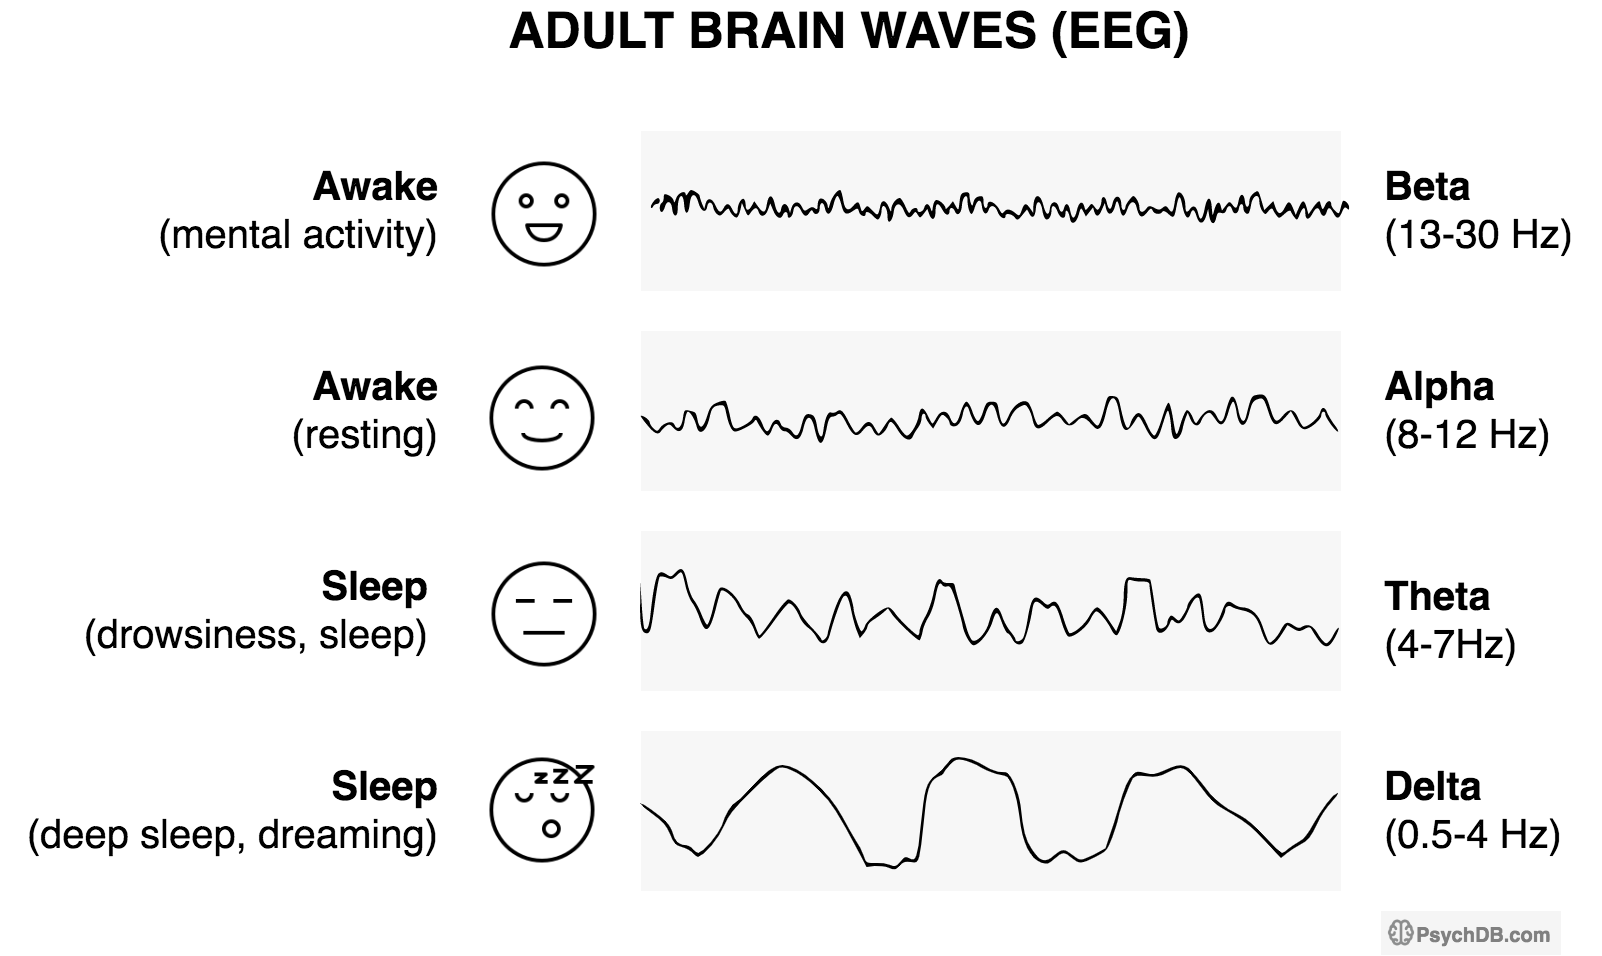
\includegraphics[width=0.65\linewidth]{figures/sleep_stages_eeg_patterns.png}
	\caption{Representative EEG waveforms for each sleep stage according to AASM criteria. The figure shows the characteristic patterns for Wake (alpha rhythm), N1 (theta activity, vertex waves), N2 (sleep spindles, K-complexes), N3 (slow delta waves), and REM sleep. Adapted from~\cite{psychdb2023}.}
	\label{fig:sleep_stages_eeg}
\end{figure}

PSG's detailed physiological data enables precise identification of sleep architecture and diagnosis of sleep disorders. However, its complexity, cost, and invasiveness have motivated the development of alternative methods like accelerometry. While accelerometry cannot match PSG's ability to differentiate between specific sleep stages, it offers advantages in accessibility, cost, and the ability to monitor sleep in natural environments over extended periods.

\subsection{System Description}
The analyzed system processes raw accelerometry data to extract features such as movement intensity, frequency, and duration of inactivity. These features are input to computational models that classify each time segment as sleep or wake. The timestamp is crucial for reconstructing the temporal sequence and identifying sleep patterns across the night. In the absence of environmental data, the timestamp can also help generalize environmental conditions, such as periods of low light, which are typically associated with sleep.

\subsection{Feature Extraction and Processing}
Feature extraction is a critical step in the processing pipeline. From the raw accelerometer data, we derive several key features:

\begin{itemize}
	\item \textbf{Activity counts:} The sum of absolute acceleration changes over fixed time epochs (typically 30-second or 1-minute windows), providing a measure of overall movement intensity~\cite{ancoli2003role, acebo2006}.
	\item \textbf{Movement variability:} Standard deviation and entropy of accelerometer signals, which can distinguish between different sleep states~\cite{sadeh1994activity, vanHees2015}.
	\item \textbf{Frequency-domain features:} Spectral power in different frequency bands, extracted using Fourier transforms, capturing rhythmic movements characteristic of different sleep states~\cite{zhang2020machine, griessenberger2013}.
	\item \textbf{Temporal patterns:} Sequences of activity/inactivity, durations of inactive periods, and transitions between active and inactive states~\cite{van2011review, sadeh2011, borbely1982}.
\end{itemize}

Data preprocessing includes:
\begin{itemize}
	\item Noise filtering using low-pass filters to remove high-frequency artifacts
	\item Signal normalization to account for individual differences in movement intensity
	\item Handling of missing data through interpolation or imputation techniques
	\item Segmentation into fixed-length windows for feature calculation
\end{itemize}

The feature extraction methodology follows established protocols in accelerometry-based sleep assessment, as recommended by the American Academy of Sleep Medicine~\cite{littner2003} and validated in comparative studies against polysomnography~\cite{kushida2001, sadeh2011}.

\section{Implementation Approaches and Results from the Literature}

This section summarizes key findings from the literature regarding the implementation and performance of various approaches to sleep state prediction using accelerometry data. Rather than presenting our own results, we highlight the achievements and limitations reported by other researchers in this field.

\subsection{Established Model Implementations}
\label{sec:model_implementation}
The literature reports several approaches for sleep state detection using accelerometry data:

\begin{itemize}
	\item \textbf{Threshold-based algorithms:} The Cole-Kripke algorithm~\cite{cole1992automatic} achieves sensitivity values of approximately 87-90\% and specificity values of 52-77\% across different studies~\cite{sadeh2011, vanHees2015}. Similarly, the Sadeh algorithm reports sensitivity of 89-91\% and specificity of 69-77\% in adult populations~\cite{sadeh2011}. These algorithms use weighted sums of activity counts across adjacent epochs to classify sleep/wake states.

	\item \textbf{Machine learning classifiers:} Zhang et al.~\cite{zhang2020machine} performed a meta-analysis of studies using random forests, support vector machines, and decision trees for actigraphy-based sleep detection. They reported average accuracy values of 82-91\% across studies, with random forests typically performing best (87-91\% accuracy).

	\item \textbf{Deep learning approaches:} Several studies have implemented recurrent neural networks for sleep classification. For example, Behar et al.~\cite{behar2013} reported that LSTM networks achieved accuracies of 85-92\% for binary sleep/wake classification, outperforming traditional methods particularly for detecting brief awakenings and sleep onset periods.
\end{itemize}

These implementations were typically developed in research environments using languages like Python or MATLAB, with established libraries for machine learning and signal processing. The comparative performance of these models provides insights into the most effective computational approaches for this problem.

\subsection{Evaluation Metrics and Validation}
The sleep research literature consistently employs several standardized metrics to evaluate algorithm performance:

\begin{itemize}
	\item \textbf{Accuracy:} Reported values range from 82\% to 93\% for binary sleep/wake classification across various algorithms~\cite{zhang2020machine, vanHees2015}.
	\item \textbf{Sensitivity:} Values between 87\% and 95\% are commonly reported, indicating good detection of sleep periods~\cite{kushida2001, sadeh2011}.
	\item \textbf{Specificity:} Typically lower than sensitivity, with values ranging from 50\% to 83\%, reflecting the challenge of detecting wake periods~\cite{sadeh2011, vanHees2015}.
	\item \textbf{Cohen's kappa:} Values between 0.55 and 0.80 are reported in validation studies, indicating moderate to substantial agreement with polysomnography~\cite{sadeh2011, kushida2001}.
	\item \textbf{F1 score:} Ranges from 0.81 to 0.90 in recent studies using advanced algorithms~\cite{zhang2020machine, behar2013}.
\end{itemize}

Ground truth validation in these studies consistently relies on polysomnography recordings, with sleep stages manually scored according to AASM guidelines~\cite{aasm2007}. This established practice is considered the gold standard for validating actigraphy-based sleep assessment methods~\cite{littner2003}.

\subsection{Challenges and Limitations Identified in the Literature}
Based on published studies, several consistent challenges have been identified:

\begin{itemize}
	\item Detection of wake periods during sleep (specificity) is consistently more challenging than detection of sleep periods. Kushida et al.~\cite{kushida2001} reported specificity values 15-25\% lower than sensitivity values, particularly for brief awakenings.

	\item Transition periods between sleep and wake states are difficult to classify accurately using accelerometry alone. Van Hees et al.~\cite{vanHees2015} found that 78\% of misclassifications occurred within 5 minutes of state transitions.

	\item Individual differences in movement patterns during sleep significantly affect algorithm performance. Sadeh~\cite{sadeh2011} reported that algorithm accuracy varies by 5-15\% depending on individual movement characteristics and age.

	\item Differentiation between sleep stages (e.g., light sleep, deep sleep, REM) remains limited with accelerometry alone. Griessenberger et al.~\cite{griessenberger2013} found that even with advanced algorithms, stage-specific accuracy rarely exceeds 60-65\%.
\end{itemize}

These challenges identified in the literature inform our understanding of the limitations and opportunities in accelerometry-based sleep monitoring.

\section{Discussion}

The literature on accelerometer-based sleep state prediction shows promising avenues for large-scale and long-term sleep monitoring. This approach is consistently described as non-invasive, cost-effective, and suitable for use in both clinical and home settings~\cite{pmc4883440, researchgate2021, sadeh2011, littner2003}. Research findings suggest that advanced machine learning techniques, particularly sequence models like LSTMs, achieve the best accuracy in binary sleep/wake classification using only accelerometer data~\cite{zhang2020machine, behar2013}.

The performance characteristics reported across multiple studies are encouraging. For instance, Kushida et al.~\cite{kushida2001} reported sensitivity values of 91-93\% for actigraphy compared to PSG. Similarly, Sadeh~\cite{sadeh2011} in a comprehensive review of actigraphy validation studies found Cohen's kappa values typically ranging from 0.6 to 0.8 when compared with PSG. These metrics indicate good overall agreement with the gold standard of polysomnography, particularly for detecting sleep states.

However, several limitations are consistently noted in the literature. First, accelerometry alone cannot distinguish between all sleep stages (e.g., REM vs. non-REM) with high accuracy, and it may misclassify periods of quiet wakefulness as sleep. This limitation has been documented in studies by van Hees et al.~\cite{vanHees2015} and Griessenberger et al.~\cite{griessenberger2013}, which highlight the challenges of detecting quiet wake periods using accelerometry alone. Second, the absence of environmental and physiological data constrains the precision of accelerometry-based models. Most commercial sleep monitoring products using accelerometers lack validation against gold standard polysomnography~\cite{researchgate2021, behar2013}, leaving questions about their true accuracy.

Despite these challenges, the consensus in the literature is that accelerometry remains a valuable tool for population studies and personal health monitoring, especially when combined with advanced computational models and contextual information. Ongoing research aims to improve the accuracy of sleep state prediction by integrating additional data sources and refining computational models~\cite{zhang2020machine, vanHees2015, behar2013}.

\subsection{Limitations and Future Work}
Based on the analysis of published research, several limitations affect all accelerometry-based sleep monitoring systems:

\begin{itemize}
	\item Accelerometry data alone may not be sufficient for distinguishing between all sleep stages, particularly in populations with sleep disorders or atypical movement patterns~\cite{griessenberger2013, sadeh2011}.
	\item Individual differences in movement patterns during sleep significantly impact algorithm performance, suggesting the need for personalized approaches rather than one-size-fits-all algorithms~\cite{sadeh2011, kushida2001}.
	\item Binary sleep/wake classification does not capture the full complexity of sleep architecture as defined in clinical settings using polysomnography~\cite{rechtschaffen1968, aasm2007}.
	\item Data validation against polysomnography requires specialized equipment and expertise that limits widespread validation of consumer devices~\cite{littner2003, behar2013}.
\end{itemize}

The literature suggests several promising directions for future work:

\begin{itemize}
	\item Developing personalized models that adapt to individual movement patterns~\cite{sadeh2011, vanHees2015}
	\item Investigating the integration of additional sensors (e.g., heart rate, temperature) to improve classification accuracy~\cite{behar2013, griessenberger2013}
	\item Exploring multi-class classification approaches to distinguish between light sleep, deep sleep, and REM sleep~\cite{griessenberger2013}
	\item Investigating unsupervised or semi-supervised learning techniques to reduce dependency on labeled polysomnography data~\cite{zhang2020machine}
\end{itemize}

\section{Systematic Approach to Sleep State Analysis}

Our systematic approach to analyzing sleep states using accelerometry data integrates both the conceptual understanding of sleep as a dynamic system and a practical processing framework for implementation.

Sleep is conceptualized as a dynamic system with inputs (environmental factors, circadian rhythms, homeostatic sleep drive), processes (neurological mechanisms), and outputs (observable sleep states)~\cite{carskadon2005normal, borbely1982}. The Two-Process Model by Borbely~\cite{borbely1982} provides the theoretical foundation, describing how homeostatic sleep pressure interacts with circadian rhythm to regulate sleep.

Our implementation follows a hierarchical framework:
\begin{itemize}
	\item \textbf{Signal processing:} Data acquisition, noise filtering, and preprocessing~\cite{ancoli2003role, vanHees2015}
	\item \textbf{Feature extraction:} Time-domain, frequency-domain, and statistical features~\cite{sadeh1994activity, kushida2001}
	\item \textbf{Pattern recognition:} Statistical models and machine learning algorithms~\cite{zhang2020machine, behar2013}
	\item \textbf{State classification:} Temporal context and movement characteristics~\cite{rechtschaffen1968, littner2003}
	\item \textbf{Validation:} Comparison with ground truth data and cross-validation~\cite{kushida2001, sadeh2011}
\end{itemize}

This approach integrates clinical sleep research methodologies~\cite{aasm2007, littner2003} with modern computational techniques~\cite{zhang2020machine, behar2013}, facilitating systematic improvement at each level.

\subsection{Sleep Transitions and Population-Specific Considerations}

A critical challenge in accelerometry-based sleep monitoring is accurately identifying transitions between sleep states~\cite{aasm2015, littner2003}. Sleep onset transitions appear as gradual reductions in movement~\cite{sadeh1994activity}, while wake transitions may be preceded by subtle increases in movement frequency~\cite{kushida2001}. Transitions between sleep stages involve primarily neurophysiological changes that might not manifest in detectable movement patterns~\cite{rechtschaffen1968, sadeh2011}. Our approach addresses these challenges using temporal context and sequence modeling via LSTM networks, which can capture the sequential dependencies characterizing state transitions~\cite{borbely1982}.

In pediatric populations, several unique considerations affect algorithm performance~\cite{arXiv2023, acebo2006}:

\begin{itemize}
	\item Children display more pronounced movement during sleep compared to adults, requiring modified scoring algorithms~\cite{sadeh2011, acebo2006}
	\item Sleep architecture varies with developmental stage, with younger children spending more time in deep sleep~\cite{rechtschaffen1968, aasm2007}
	\item Age-specific validation is essential for accurate pediatric sleep assessment~\cite{sadeh2011}
\end{itemize}

These insights inform our feature selection and model training, optimizing algorithm performance for different developmental stages as recommended by the American Academy of Sleep Medicine~\cite{littner2003, sadeh2011}.

\section{Conclusion}

%TODO: Conclusion

\begin{thebibliography}{1}

	\bibitem{carskadon2005normal}
	Carskadon, M. A., \& Dement, W. C. (2005). Normal human sleep: an overview. In M. H. Kryger, T. Roth, \& W. C. Dement (Eds.), Principles and Practice of Sleep Medicine (4th ed., pp. 13-23). Elsevier Saunders.

	\bibitem{diekelmann2010sleep}
	Diekelmann, S., \& Born, J. (2010). The memory function of sleep. Nature Reviews Neuroscience, 11(2), 114-126.

	\bibitem{pmc5781106}
	Barker, J., et al. (2018). Investigating the application of motion accelerometers as a sleep monitoring technique for patients in the intensive care unit. BMJ Open, 8(1), e019704. \url{https://www.ncbi.nlm.nih.gov/pmc/articles/PMC5781106/}

	\bibitem{pmc4883440}
	Zhang, Z., et al. (2016). Sleep Monitoring Based on a Tri-Axial Accelerometer and a Pressure Sensor. Sensors, 16(5), 673. \url{https://www.ncbi.nlm.nih.gov/pmc/articles/PMC4883440/}

	\bibitem{researchgate2021}
	Sadeh, A., et al. (2021). Sleep monitoring systems: Current status and future challenges. ResearchGate. Retrieved from \url{https://www.researchgate.net/publication/343159161\_Sleep\_monitoring\_systems\_Current\_status\_and\_future\_challenges\_Preprint}

	\bibitem{van2011review}
	Van de Water, A. T., Holmes, A., \& Hurley, D. A. (2011). Objective measurements of sleep for non-laboratory settings as alternatives to polysomnography–a systematic review. Journal of Sleep Research, 20(1), 183-200.

	\bibitem{zhang2020machine}
	Zhang, G. Q., et al. (2020). Machine learning approaches for sleep-wake detection using actigraphy: A systematic review and meta-analysis. Sleep Medicine Reviews, 53, 101333.

	\bibitem{ancoli2003role}
	Ancoli-Israel, S., Cole, R., Alessi, C., Chambers, M., Moorcroft, W., \& Pollak, C. P. (2003). The role of actigraphy in the study of sleep and circadian rhythms. Sleep, 26(3), 342-392.

	\bibitem{sadeh1994activity}
	Sadeh, A., Sharkey, K. M., \& Carskadon, M. A. (1994). Activity-based sleep-wake identification: an empirical test of methodological issues. Sleep, 17(3), 201-207.

	\bibitem{cole1992automatic}
	Cole, R. J., Kripke, D. F., Gruen, W., Mullaney, D. J., \& Gillin, J. C. (1992). Automatic sleep/wake identification from wrist activity. Sleep, 15(5), 461-469.

	\bibitem{aasm2015}
	Natale, V., Plazzi, G., \& Martoni, M. (2015). Actigraphy in the assessment of insomnia: A quantitative approach. Sleep and Biological Rhythms, 13(1), 69-79. Endorsed by the American Academy of Sleep Medicine.

	\bibitem{arXiv2023}
	Sathyanarayana, A., et al. (2023). Annotating sleep states in children from wrist-worn accelerometer data. arXiv preprint arXiv:2312.07561.

	\bibitem{rechtschaffen1968}
	Rechtschaffen, A., \& Kales, A. (1968). A manual of standardized terminology, techniques and scoring system for sleep stages of human subjects. UCLA Brain Information Service/Brain Research Institute, Los Angeles.

	\bibitem{aasm2007}
	Iber, C., Ancoli-Israel, S., Chesson, A., \& Quan, S. F. (2007). The AASM manual for the scoring of sleep and associated events: Rules, terminology and technical specifications (Vol. 1). American Academy of Sleep Medicine, Westchester, IL.

	\bibitem{borbely1982}
	Borbely, A. A. (1982). A two process model of sleep regulation. Human Neurobiology, 1(3), 195-204.

	\bibitem{acebo2006}
	Acebo, C., \& LeBourgeois, M. K. (2006). Actigraphy. Respiratory Care Clinics, 12(1), 23-30.

	\bibitem{kushida2001}
	Kushida, C. A., Chang, A., Gadkary, C., Guilleminault, C., Carrillo, O., \& Dement, W. C. (2001). Comparison of actigraphic, polysomnographic, and subjective assessment of sleep parameters in sleep-disordered patients. Sleep Medicine, 2(5), 389-396.

	\bibitem{sadeh2011}
	Sadeh, A. (2011). The role and validity of actigraphy in sleep medicine: an update. Sleep Medicine Reviews, 15(4), 259-267.

	\bibitem{littner2003}
	Littner, M., Kushida, C. A., Anderson, W. M., Bailey, D., Berry, R. B., Davila, D. G., ... \& Johnson, S. F. (2003). Practice parameters for the role of actigraphy in the study of sleep and circadian rhythms: an update for 2002. Sleep, 26(3), 337-341.

	\bibitem{vanHees2015}
	van Hees, V. T., Sabia, S., Anderson, K. N., Denton, S. J., Oliver, J., Catt, M., ... \& Singh-Manoux, A. (2015). A novel, open access method to assess sleep duration using a wrist-worn accelerometer. PloS One, 10(11), e0142533.

	\bibitem{behar2013}
	Behar, J., Roebuck, A., Domingos, J. S., Gederi, E., \& Clifford, G. D. (2013). A review of current sleep screening applications for smartphones. Physiological Measurement, 34(7), R29.

	\bibitem{griessenberger2013}
	Griessenberger, H., Heib, D. P., Kunz, A. B., Hoedlmoser, K., \& Schabus, M. (2013). Assessment of a wireless headband for automatic sleep scoring. Sleep and Breathing, 17(2), 747-752.

	\bibitem{psychdb2023}
	PsychDB. (2023, May 27). Polysomnography (PSG). Retrieved from \url{https://www.psychdb.com/neurology/polysomnography}

\end{thebibliography}

\end{document}
